% !TEX root = ../main.tex

\chapter{Measurement Principle}
\label{ch:measurement-principle}

\scaffold{
  Chapter purpose: the theory the implementation rests on, independent of the concrete chips. The reader knows from \cref{ch:introduction} that the wiring of a pedal is unknown and from \cref{sec:related-component-identification} that component testers drive pins through resistors. By the end of the chapter the reader can compute the arm resistances of any pedal from three contact voltages per drive pair, knows why every tolerance is a multiple of the ADC noise, and knows how a plug is detected and an identified pedal is followed. Values of the board (\qty{1}{\kilo\ohm}, \qty{2.5}{\volt}) appear only as examples; the board itself follows in \cref{ch:implementation}.
}

% !TEX root = ../main.tex

\section{Expression Pedal Wiring}
\label{sec:pedal-wiring}

\scaffold{
  \textbf{Paragraph 1.} Link: \cref{ch:introduction} named the two common wirings. Show them in \cref{fig:pedal-wirings} and name each panel: wiper on the tip with ring as reference and sleeve as ground, wiper on the ring with tip as reference \cite{mission2014expression, nonlinearlabs2026pedals}, and the two-wire variants that connect only tip and sleeve. Point out that the sleeve is a track end in both common three-wire wirings; \cref{sec:following} builds the position convention on this.
}

\begin{figure}[htbp]
  \centering
  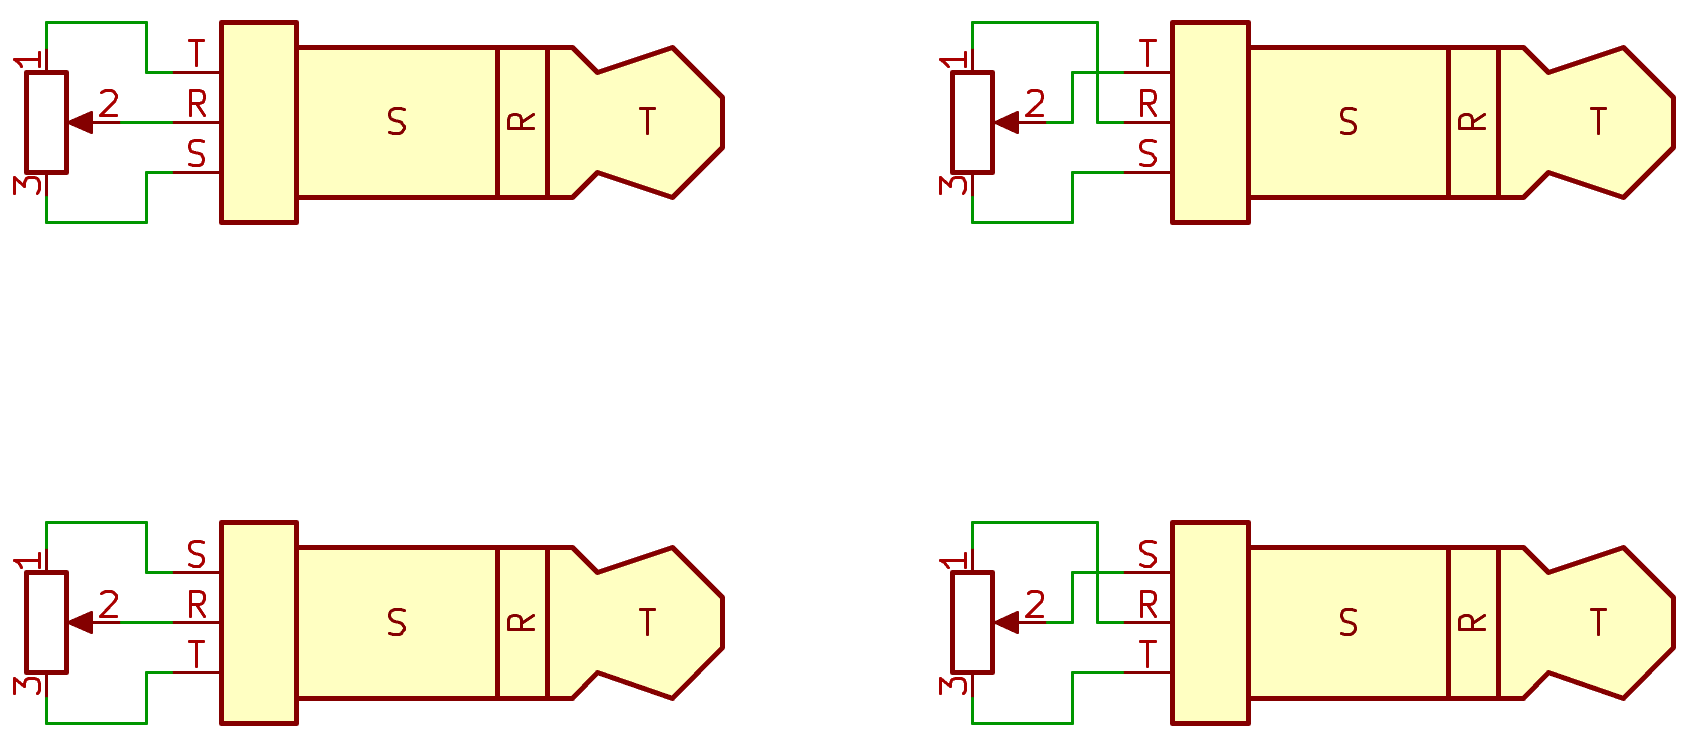
\includegraphics[width=0.85\linewidth]{03-measurement-principle/figures/pedal-wirings}
  \titledcaption{Expression Pedal Wirings}{\scaffoldinline{Name the four panels (which contact carries the wiper, which end goes to the sleeve, which variant is two-wire) and say that the potentiometer symbol is the pedal and the plug drawing the TRS plug. Source: drawing from the final presentation; check whether the four panels match the four cases named in the text, otherwise redraw.}}
  \label{fig:pedal-wirings}
\end{figure}

\scaffold{
  \textbf{Paragraph 2, pedal types and plugs.} Besides potentiometer pedals, the interface accepts sustain switches and two-wire rheostats. Which contacts conduct depends on the plug: a mono (TS) plug shorts the jack's ring contact to its sleeve, a stereo (TRS) plug leaves it unconnected. \Cref{tab:pedal-networks} lists the resulting networks; it is the reference the classification in \cref{sec:following} checks against.
}

\begin{table}[htbp]
  \centering
  \titledcaption{Pedal Networks Behind Mono and Stereo Plugs}{\scaffoldinline{Explain that each cell names which jack contacts conduct; source: \code{docs/fast-tracking.md} of the project repository.}}
  \label{tab:pedal-networks}
  \begin{tabularx}{\linewidth}{@{}l>{\raggedright\arraybackslash}X>{\raggedright\arraybackslash}X@{}}
    \toprule
    \textbf{Pedal} & \textbf{Mono plug (TS)} & \textbf{Stereo plug (TRS)} \\
    \midrule
    Potentiometer & track halves in parallel (see text) & three arms, wiper near the star point \\
    Switch, released & tip open, ring and sleeve shorted & nothing conducts \\
    Switch, pressed & all contacts shorted & tip and sleeve shorted, ring open \\
    Rheostat & tip carries it, ring and sleeve shorted & tip and sleeve carry it, ring open \\
    Cable without pedal & as a released switch & nothing conducts \\
    \bottomrule
  \end{tabularx}
\end{table}

\scaffold{
  \textbf{Paragraph 3, the mono-cable limit.} Most pedals' own jacks short their ring terminal to the sleeve when a mono plug is inserted. For a potentiometer this puts the two track halves in parallel, which gives the resistance $R\,x(1-x)$ at travel $x$ for a track of $R$: zero at both ends and $R/4$ in the middle. Derive this in one line. Conclude that the position cannot be recovered from any measurement, so potentiometer pedals need a stereo cable; this is a property of the pedal, not of the interface.
}

% !TEX root = ../main.tex

\section{Star Network Model}
\label{sec:star-network}

\scaffold{
  \textbf{Paragraph 1, the model.} Every pedal of \cref{sec:pedal-wiring} is a passive network between three terminals. Any such network is externally equivalent to three resistors meeting in one inner node, the star point \cite{kennelly1899equivalence}, as drawn in \cref{fig:star-network}. Define the term \emph{arm}: the resistance between one contact and the star point, written $r_\mathrm{T}$, $r_\mathrm{R}$ and $r_\mathrm{S}$ for tip, ring and sleeve. Use \enquote{arm} throughout, never \enquote{branch} or \enquote{leg}. State that the internal topology cannot be recovered from the terminals, only this equivalent \cite{borcea2012resistor}; the star form is chosen over the triangle form because, with one terminal open, a pair resistance is simply the sum of two arms.
}

\begin{figure}[htbp]
  \centering
  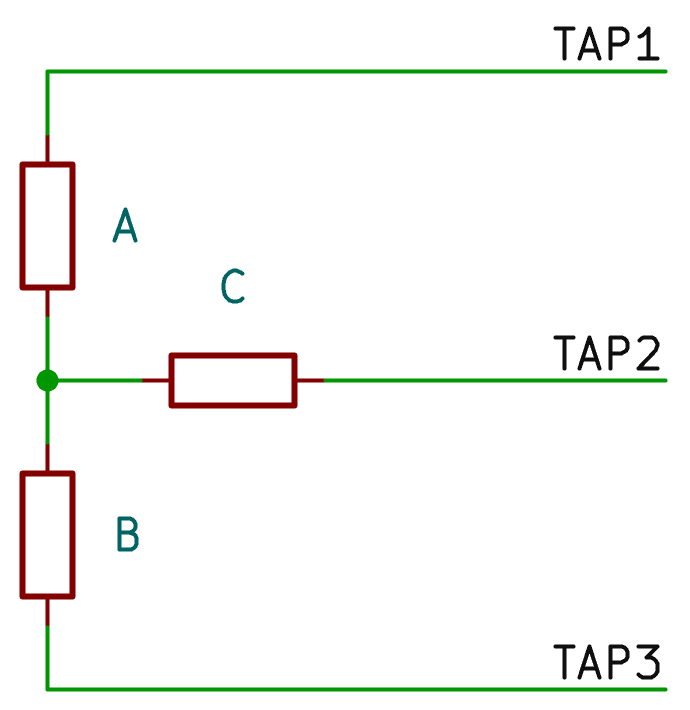
\includegraphics[width=0.3\linewidth]{03-measurement-principle/figures/star-network}
  \titledcaption{Star Network Model}{\scaffoldinline{Say that A, B and C are the three arms meeting in the star point and TAP1 to TAP3 the accessible contacts. Consider redrawing with the labels of the text ($r_\mathrm{T}$, $r_\mathrm{R}$, $r_\mathrm{S}$; tip, ring, sleeve), so that figure and text use one notation.}}
  \label{fig:star-network}
\end{figure}

\scaffold{
  \textbf{Paragraph 2, what the arms mean.} Translate the pedal types into arm values: a potentiometer is the case with exactly one arm near \qty{0}{\ohm}, the wiper, while the other two arms hold the two track sections; the ratio of these two is the position. A wiper resting on a track end additionally shorts that end to the star point (end stop). A two-wire pedal has an isolated arm. Conclude: identifying a pedal reduces to solving for three arm resistances and asking which are near zero or isolated.
}

\scaffold{
  \textbf{Paragraph 3, representation.} The solver reports the arms as relative values $q_i = r_i / R_\mathrm{tot}$ (summing to one) plus the total $R_\mathrm{tot} = \sum_i r_i$, because the ratios are measured far more precisely than the total (\cref{sec:pair-measurement}). Special values use the IEEE~754 encoding: $0$ for an arm shorted to the star point, $\infty$ for an isolated arm, NaN for an arm that is finite but cannot be separated from its partner, which happens when only two contacts are connected. Mention that this keeps the arithmetic closed, so no special cases propagate through the code.
}

% !TEX root = ../main.tex

\section{Pair Measurement}
\label{sec:pair-measurement}

\scaffold{
  \textbf{Paragraph 1, the drive states.} The star point is not accessible, so the arms have to be inferred from the contacts. Every contact can be connected to a pull-up resistor to the high rail, to a pull-down resistor to the low rail, or left floating, and every contact is read by the ADC (\cref{fig:pull-matrix}). Define the term \emph{reading}: one settled ADC result of one contact; its cost in time follows in \cref{sec:conversion}. Define the term \emph{drive} (high, low, floating) and the term \emph{pull resistance} $R_\mathrm{p}$; on this board $R_\mathrm{p} = \qty{1}{\kilo\ohm}$ for both rails. Define \emph{rail voltages} $V_{\mathrm{H},i}$ and $V_{\mathrm{L},i}$: what contact $i$ reads when it is driven high or low while no current flows. They are measured, not assumed, by driving all three arms to the same rail and averaging eight readings per arm; this cancels the offset of the ADC and the voltage drops of the switches.
}

\begin{figure}[htbp]
  \centering
  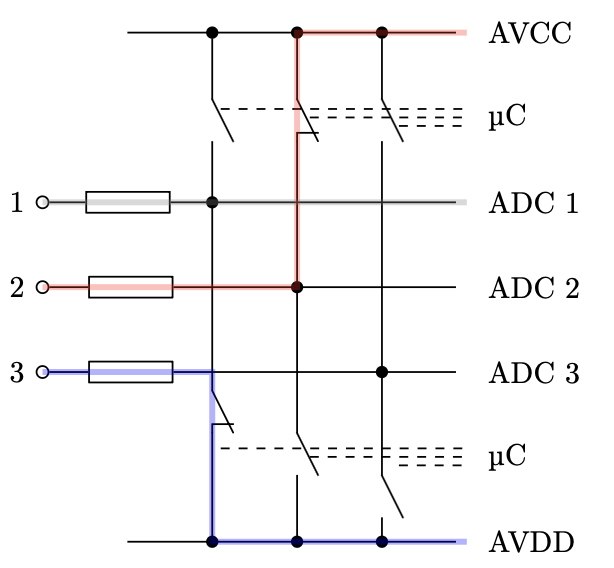
\includegraphics[width=0.45\linewidth]{03-measurement-principle/figures/pull-matrix}
  \titledcaption{Pull Matrix}{\scaffoldinline{Explain the three switch columns per contact (to the high rail, to the low rail, each controlled by the microcontroller), the series resistor at each contact and the ADC channel per contact. The highlighted example drives contact 2 high and contact 3 low while contact 1 floats. Note that the figure labels the rails AVCC and AVDD; in the text they are the high and low rail.}}
  \label{fig:pull-matrix}
\end{figure}

\scaffold{
  \textbf{Paragraph 2, one pair.} A \emph{pair measurement} drives one arm $h$ high and one arm $l$ low and leaves the third arm $f$ floating, then reads all three contacts. The floating contact carries no current, so it reads the star point voltage. Present \cref{eq:currents,eq:pair-resistance,eq:low-fraction} in this order and explain each in one sentence: the loop current seen on the high and on the low side, the resistance of the pair, and the share of the pair held by the low arm. Point out that \cref{eq:low-fraction} uses voltages only, which span most of the rail, while \cref{eq:currents} relies on the small drops across the pull resistors; this is why ratios are precise and the total is not.
}

\begin{align}
  I_\mathrm{H} &= \frac{V_{\mathrm{H},h} - V_h}{R_\mathrm{p}},
  \qquad
  I_\mathrm{L} = \frac{V_l - V_{\mathrm{L},l}}{R_\mathrm{p}},
  \qquad
  I = \frac{I_\mathrm{H} + I_\mathrm{L}}{2}
  \label{eq:currents} \\
  R_{hl} &= r_h + r_l = \frac{V_h - V_l}{I}
  \label{eq:pair-resistance} \\
  \rho_{hl} &= \frac{V_f - V_l}{V_h - V_l} = \frac{r_l}{r_h + r_l}
  \label{eq:low-fraction}
\end{align}

\scaffold{
  \textbf{Paragraph 3, consistency and conduction.} $I_\mathrm{H}$ and $I_\mathrm{L}$ are two readings of the same loop current, so their difference is a free consistency check: a pedal moved during the measurement, or an unsettled contact, shows up as disagreement. A pair conducts only if both driven arms are finite; an isolated arm leaves $I$ at zero within the noise. Refer forward to \cref{sec:tolerances} for the thresholds of both checks.
}

\scaffold{
  \textbf{Paragraph 4, worked example.} Walk through \cref{fig:topology-sim-pairs}: the simulator of milestone~2 \cite{benson2026topologysim} with arms of 100, 200 and \qty{300}{\kilo\ohm} and \qty{1}{\kilo\ohm} pulls. In (a), the first pair puts the floating contact at \qty{1.66}{\volt}, i.e. 67\,\% of the span; in (b) the second pair puts it at \qty{1.87}{\volt}, 75\,\%. Compute both ratios with \cref{eq:low-fraction} to show the reader the arithmetic once. Mention that the simulator assumes a \qty{2.5}{\volt} rail.
}

\begin{figure}[htbp]
  \centering
  \begin{subfigure}[t]{0.49\linewidth}
    \centering
    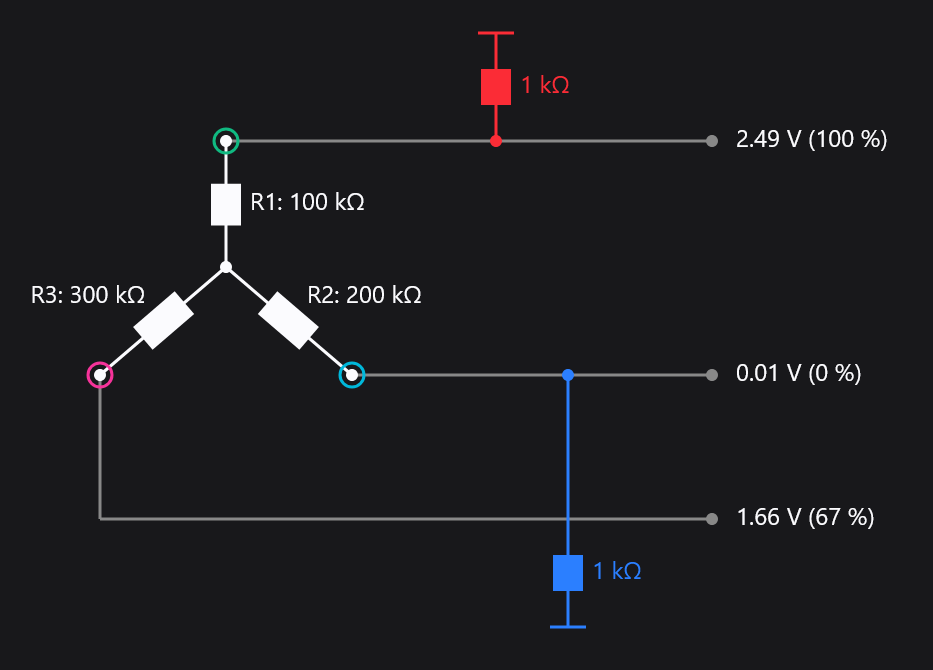
\includegraphics[width=\linewidth]{03-measurement-principle/figures/topology-sim-first-pair}
    \caption{First Pair}
    \label{fig:topology-sim-first-pair}
  \end{subfigure}%
  \hfill%
  \begin{subfigure}[t]{0.49\linewidth}
    \centering
    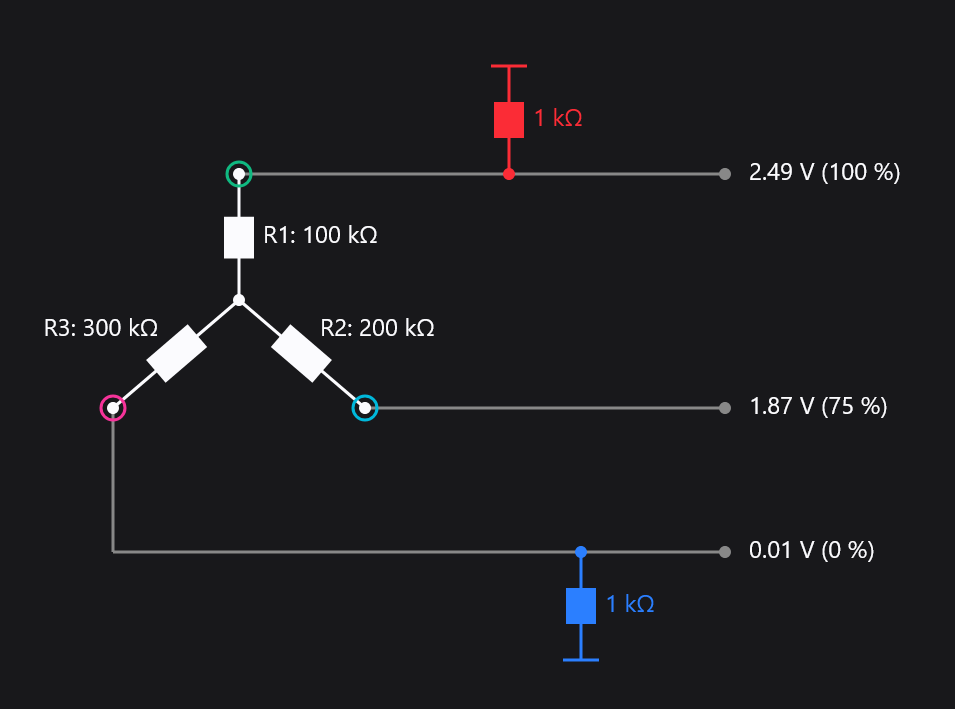
\includegraphics[width=\linewidth]{03-measurement-principle/figures/topology-sim-second-pair}
    \caption{Second Pair}
    \label{fig:topology-sim-second-pair}
  \end{subfigure}
  \titledcaption{Pair Measurements in the Simulator}{\scaffoldinline{State the network (R1 \qty{100}{\kilo\ohm}, R2 \qty{200}{\kilo\ohm}, R3 \qty{300}{\kilo\ohm}), mark which contact is pulled up (red) and down (blue) in (a) and (b), and read off the floating contact voltage in each. Screenshots of \cite{benson2026topologysim}; verify that the arm labels match the text before use.}}
  \label{fig:topology-sim-pairs}
\end{figure}

% !TEX root = ../main.tex

\section{Solving the Network}
\label{sec:solving}

\scaffold{
  \textbf{Paragraph 1, the sequence.} Define the term \emph{solve}: the sequence of pair measurements that determines all three arms, and its result. One pair yields two independent numbers (a ratio and a resistance), the network has three unknowns, so at least two pairs are needed. The solver measures the pairs (tip high, ring low), (tip high, sleeve low) and, only if needed, (ring high, sleeve low). The first two share the tip, so only the low side has to be switched between them. The third pair is needed when neither of the first two conducts (an isolated tip and an empty plug look the same to them) or when the shared arm is too close to \qty{0}{\ohm} (paragraph 3).
}

\scaffold{
  \textbf{Paragraph 2, ratios through a shared arm.} Two pairs that share arm $s$, one with arm $a$ and one with arm $b$, give the shares $\sigma_1 = r_s/(r_s + r_a)$ and $\sigma_2 = r_s/(r_s + r_b)$ from \cref{eq:low-fraction}. Present \cref{eq:ratios}: the three unnormalized ratios $x_i$ and the relative arms $q_i$. Derive in one step that each $x_i$ is proportional to $r_i$ with the common factor in \cref{eq:conditioning}, so the normalization recovers the arms exactly.
}

\begin{align}
  x_s &= \sigma_1 \sigma_2, \qquad
  x_a = (1 - \sigma_1)\,\sigma_2, \qquad
  x_b = (1 - \sigma_2)\,\sigma_1, \qquad
  q_i = \frac{x_i}{\sum_j x_j}
  \label{eq:ratios} \\
  c &= \sum_j x_j = \frac{r_s\,(r_s + r_a + r_b)}{(r_s + r_a)(r_s + r_b)}
  \label{eq:conditioning}
\end{align}

\scaffold{
  \textbf{Paragraph 3, conditioning.} Define the \emph{conditioning} $c$ of \cref{eq:conditioning}: it lies between 0 and 1 and approaches 0 as the shared arm approaches \qty{0}{\ohm}, because both pairs then only say \enquote{everything is in the other arm}. Noise in the ratios is amplified roughly by $1/c$. This is exactly the case of a potentiometer whose wiper is the tip: with a contact resistance $t$ of the wiper, $c \approx t/((t + r)(t + s))$ in relative terms. Below a minimum conditioning of 0.5 the solver measures the third pair and takes the better conditioned of its two combinations. Refer to \cref{sec:update-rate}, where a threshold of 0.05 let a pedal with a \qty{1.5}{\percent} wiper pass and its position jitter by \num{4880} instead of \num{274} parts per million.
}

\scaffold{
  \textbf{Paragraph 4, the total.} Each conducting pair $k$ implies a total $R_{\mathrm{tot},k} = R_{hl,k} / (q_h + q_l)$. The solver combines them weighted with their squared signal-to-noise ratio $I_k^2/\operatorname{Var}(I_k)$ (\cref{eq:total}). The pairs must agree on the total within their noise; a pedal moved between two pairs does not, and the solve is rejected and repeated.
}

\begin{equation}
  R_\mathrm{tot} = \frac{\sum_k w_k R_{\mathrm{tot},k}}{\sum_k w_k},
  \qquad
  w_k = \frac{I_k^2}{\operatorname{Var}(I_k)}
  \label{eq:total}
\end{equation}

\scaffold{
  \textbf{Paragraph 5, degenerate networks.} A pair whose resistance is below \qty{50}{\ohm} is a short: if both of the first pairs are shorts, every arm is 0; if one is, the remaining arm holds the whole resistance. If exactly one pair conducts, the third arm is isolated and the two conducting arms are either both shorted or only known as a sum (NaN, \cref{sec:star-network}). If no pair conducts, the network is disconnected. This covers every case of \cref{tab:pedal-networks}.
}

% !TEX root = ../main.tex

\section{Tolerances from the ADC Noise}
\label{sec:tolerances}

\scaffold{
  \textbf{Paragraph 1, the principle.} Every threshold of the solver is expressed in standard deviations of the noise of a single ADC reading, $\sigma_V$, propagated to the quantity that is checked: a current read across $R_\mathrm{p}$ has $\operatorname{Var}(I_\mathrm{H}) = (\sigma_V / R_\mathrm{p})^2$, the averaged current a quarter of the sum of both sides. Consequence: a high-value pedal, whose small currents are noisy, gets proportionally wider tolerances instead of being rejected, and adapting the solver to another front end only requires its $\sigma_V$. On this board $\sigma_V = \qty{0.5}{\milli\volt}$ at the chosen update rate (\cref{sec:update-rate}). Note the history: the first version used exact-arithmetic thresholds from the simulator ($10^{-9}$) that rejected every real measurement.
}

\scaffold{
  \textbf{Paragraph 2, the thresholds.} Present \cref{tab:solver-tolerances} and comment on the two that matter most: the conduction threshold of $3\sigma$ decides the largest pair resistance still distinguishable from an open circuit, and the minimum conditioning (\cref{sec:solving}) decides when a third pair is measured. Compute once what the conduction threshold means in resistance for $R_\mathrm{p} = \qty{1}{\kilo\ohm}$ and a \qty{2.5}{\volt} rail.
}

\begin{table}[htbp]
  \centering
  \titledcaption{Solver Tolerances}{\scaffoldinline{Say that $\sigma$ is the noise of the checked quantity derived from $\sigma_V$, that a check passes if either the noise criterion or the relative criterion holds, and give the source (\code{SolverConfig::from\_voltage\_noise} in \code{topology/src/config.rs}).}}
  \label{tab:solver-tolerances}
  \begin{tabular}{@{}lll@{}}
    \toprule
    \textbf{Check} & \textbf{Noise criterion} & \textbf{Relative criterion} \\
    \midrule
    Pair conducts & $I > 3\sigma_I$ & -- \\
    High and low current agree & $5\sigma$ & \qty{10}{\percent} of $I$ \\
    Pair totals agree & $4\sigma$ & \qty{10}{\percent} of $R_\mathrm{tot}$ \\
    Pair is a short & -- & $R_{hl} < \qty{50}{\ohm}$ \\
    Ratio is defined & $V_h - V_l > 10\sigma_V$ & -- \\
    Two pairs suffice & -- & conditioning $c \geq 0.5$ \\
    \bottomrule
  \end{tabular}
\end{table}

% !TEX root = ../main.tex

\section{Plug Detection}
\label{sec:plug-detection}

\scaffold{
  \textbf{Paragraph 1, why a separate check.} A solve cannot tell an empty jack from a plugged cable with nothing conducting behind it, since both leave every pair open. The jacks have a fourth contact for this: the \emph{tip switch}, a normalling contact that touches the tip while no plug is inserted and is lifted by the plug \cite{neutrik2026nmj6hfd2}. Use the term \enquote{tip switch} throughout, never \enquote{normalling contact} after its definition.
}

\scaffold{
  \textbf{Paragraph 2, the check.} The \emph{plug check} drives the tip low and the tip switch high and leaves ring and sleeve floating. Without a plug the two pulls form a divider and the tip switch reads half the rail span, \qty{1.25}{\volt}; with a plug it is isolated and reads its own rail, \qty{2.5}{\volt}. A plug is assumed above three quarters of the span (\cref{eq:plug-threshold}). Explain why the check is independent of the pedal: ring and sleeve float, so no current flows through the pedal whatever its wiring, position or end stop, including a wiper on the tip. It costs one reading plus the re-settling of whatever the jack was driven with before.
}

\begin{equation}
  V_\mathrm{TS} > V_{\mathrm{L},\mathrm{TS}} + 0.75\,\bigl(V_{\mathrm{H},\mathrm{TS}} - V_{\mathrm{L},\mathrm{TS}}\bigr)
  \label{eq:plug-threshold}
\end{equation}

\scaffold{
  \textbf{Paragraph 3, origin of the fourth contact.} One sentence for the reader: the board switches four contacts per jack because the switch ICs have four channels, and the spare channel was put on the tip switch (author's statement in the final presentation); the use for plug detection followed from that. Refer to \cref{sec:design-history}.
}

% !TEX root = ../main.tex

\section{Following an Identified Pedal}
\label{sec:following}

\scaffold{
  \textbf{Paragraph 1, why following.} A full solve takes two or three pairs of three readings each. For an identified potentiometer, a single reading suffices: once the wiper and the track ends are known, the track ends are driven and only the wiper is read. The wiper then carries no current, so its contact resistance does not enter the position. Present \cref{eq:position}, with $V_\mathrm{s}$ and $V_\mathrm{e}$ the readings of the track start and end. Leave the timing argument (why this is necessary) to \cref{sec:update-rate}.
}

\begin{equation}
  p = \frac{V_\mathrm{w} - V_\mathrm{s}}{V_\mathrm{e} - V_\mathrm{s}}, \qquad 0 \leq p \leq 1
  \label{eq:position}
\end{equation}

\scaffold{
  \textbf{Paragraph 2, position convention.} The track start is the sleeve whenever the sleeve is a track end, otherwise the lower-numbered end. With this, the position rises as the wiper moves away from the sleeve, which matches both common wirings of \cref{fig:pedal-wirings}. Mention that the first firmware counted from the lower-numbered end and read the tip-wiper test pedal backwards.
}

\scaffold{
  \textbf{Paragraph 3, classification.} After a solve, the arms decide what follows. Walk through the classes in the order they are checked, with their thresholds relative to $R_\mathrm{tot}$:
  \emph{potentiometer} (every arm resolved, exactly one within \qty{25}{\percent}: the wiper);
  \emph{end stop} (two arms within \qty{2}{\percent}: the wiper rests on a track end);
  \emph{near end} (the second-lowest arm also within \qty{25}{\percent});
  \emph{tip-sleeve element} (a switch or rheostat behind a mono or stereo plug, \cref{tab:pedal-networks});
  \emph{disconnected}; and \emph{other} for any remaining network, such as a dual footswitch.
  Explain the ambiguity of end stop and near end: a clean wiper a little way along the track and a wiper with resistance in its own lead resting on that end are the same network at opposite positions; only the ring-sleeve end stop changes the position. The wiper is then taken from, in this order, the per-jack wiper setting, the wiper remembered for the jack, and the arm nearer the star point unless that is the sleeve. Refer to \cref{sec:pedal-types} for the pedal that required the \qty{25}{\percent} limit.
}

\scaffold{
  \textbf{Paragraph 4, checks while following a potentiometer.} Every \qty{25}{\milli\second} one track end is read instead of the wiper, alternating. Its drop across the pull resistor must stay within $6\sigma$ or \qty{3}{\percent} of the reference (\qty{25}{\percent} on the very first reading, because solves of a pedal on an end stop were seen up to \qty{10}{\percent} off). The wiper must stay within the span of the ends, with $6\sigma$ plus \qty{0.5}{\percent} of the span as margin (a pedal read its wiper up to \qty{7}{\milli\volt} past the end it rested on). A violation means the pedal was unplugged, rewired, or its wiper guessed wrong, and the jack is identified again.
}

\scaffold{
  \textbf{Paragraph 5, switches and rheostats.} A tip-sleeve element is followed with one reading as well: tip high, sleeve low, tip read; the resistance follows from the tip's pull drop. At most \qty{0.2}{\kilo\ohm} reads as a closed switch (value 1), no current as open (value 0); three consecutive readings in between make it a rheostat, whose resistance is scaled to the smallest standard pedal value (1, 2.5, 5, 10, 25 \ldots\ \qty{1000}{\kilo\ohm}) it fits within \qty{25}{\percent}. A plug check every \qty{50}{\milli\second} and a ring check every \qty{100}{\milli\second} confirm the plug is still there and the ring still wired as identified; the ring check allows \qty{1}{\percent} of the sleeve's drop on top of $6\sigma$ because the two pull paths differ by a few ohms. State the two known limitations: a mono cable without a pedal reads as a released switch, and a rheostat behind a mono plug first reads as a potentiometer on its end stop until its resistance has changed by \qty{20}{\percent}.
}

